%%
%% This is file `chapmin.tex',
%% generated with the docstrip utility.
%%
%% The original source files were:
%%
%% ths.dtx  (with options: `chapmin')
%% 
%% IMPORTANT NOTICE:
%% 
%% For the copyright see the source file.
%% 
%% Any modified versions of this file must be renamed
%% with new filenames distinct from chapmin.tex.
%% 
%% For distribution of the original source see the terms
%% for copying and modification in the file ths.dtx.
%% 
%% This generated file may be distributed as long as the
%% original source files, as listed above, are part of the
%% same distribution. (The sources need not necessarily be
%% in the same archive or directory.)

This chapter summarizes the solution methodology employed by DOCTORS. The techniques used to compute the collided and uncollided fluxes are described in seperate sections. After the flux solution methodology is explained, the methods used for source generation and flux-to-dose conversion are covered.

\section{Discrete Ordinate Methods}

The discrete ordinate solver computes the flux distribution inside the CT mesh given a source, physical geometry information, and other associated solver parameters such as quadrature and energy discretization. Discrete ordinates is a deterministic solution to the linear Boltzmann equation.

\subsection{The Boltzmann Equation}

The linear Boltzmann equation (LBE) is generally true of any particle given that outside forces (electromagnetic or graitational) are either not present or negligible and particle-particle collisions are insignificant. Therefore, the LBE is generally not valid for charged parpticles or systems whose particle density is on the order of the medium they are traveling trhrough. In such systems, particle-particle ineractions may not be negligible.  

In general, the LBE is valid for multiplying media (such as neutrons passing through fuel in a reactor), but the variant considered in this work omits such terms since only photons in medical systems are of concern. Solutions to the LBE can also be used to solve criticality eigenvalue problems or to produce adjoint parameters for other codes. Such solutions are not considered in this work.

\begin{equation} \label{eq:boltz_t_dep}
\begin{split}
	&\left[ \frac{1}{v(\boldsymbol{r},t)} \frac{\partial}{\partial t} + \hat{\Omega} \cdot \nabla + \Sigma_t(\boldsymbol{r}, E, t) \right]
	\psi(\boldsymbol{r}, E, \hat{\Omega}, t) = \\
	&\int_{4 \pi} \int_0^\infty \Sigma_s(\boldsymbol{r}, E' \rightarrow E, \hat{\Omega}' \rightarrow \hat{\Omega}, t) \psi(\boldsymbol{r}, E', \hat{\Omega}', t) dE' d\hat{\Omega}' + S(\boldsymbol{r}, E, \hat{\Omega}, t)
\end{split}
\end{equation}

\noindent
where $v$ is the velocity of the photon in the medium at $\boldsymbol{r}$, $\Sigma_t$ is the total macroscopic cross section, $\Sigma_s$ is the macroscopic scattering cross section, $S$ is an external photon source, and $\psi$ is the total photon angular flux. 

The transient case is not typically of interest in medical diagnostic imaging, rather the steady state is more important. The time dependence in Eq. \ref{eq:boltz_t_dep} is removed to yield

\begin{equation} \label{eq:boltz}
\begin{split}
	&\left[ \hat{\Omega} \cdot \nabla + \Sigma_t(\boldsymbol{r}, E) \right]
	\psi(\boldsymbol{r}, E, \hat{\Omega}) = \\
	&\int_{4 \pi} \int_0^\infty \Sigma_s(\boldsymbol{r}, E' \rightarrow E, \hat{\Omega}' \rightarrow \hat{\Omega}) \psi(\boldsymbol{r}, E', \hat{\Omega}') dE' d\hat{\Omega}' + S(\boldsymbol{r}, E, \hat{\Omega})
\end{split}
\end{equation}

The steady state form of the LBE can be readily derived from simple intuition. In the steady state, particle production and removal must be equal. In any volume, three production mechanisms are present. Particles can stream into the volume across a bounding surface, they can inscatter from another energy-direction component of phase space, or they can be produced directly by the external source. Three removal terms are also present, particles can stream out of the volume of interest by crossing a bounding surface, be absorbed and vanish entirely, or outscatter to a energy-direction componennt of phase space other than the one of interest.

The downscatter and absorbtiption removal terms are typically grouped together as

\begin{equation}
\Sigma_t(\boldsymbol{r}, E) \psi(\boldsymbol{r}, E, \hat{\Omega})
\end{equation}

\noindent
and both production and removal streaming operators are combined as well as

\begin{equation}
\hat{\Omega} \cdot \nabla \psi(\boldsymbol{r}, E, \hat{\Omega})
\end{equation}

\noindent
and included as a removal term since they normal is defined pointing outward from the volume. The normal sign convention results in particles streaming out being positive and those streaming in beocming negative. The inscatter to a particular energy and direction is computed by integrating over all other energies and diretions

\begin{equation}
\int_{4\pi}^{} \int_{0}^{\infty} \Sigma_s(\boldsymbol{r}, E' \rightarrow E, \hat{\Omega}' \rightarrow \hat{\Omega}) \psi(\boldsymbol{r}, E', \hat{\Omega}') dE' d\hat{\Omega}'
\end{equation}

The following sections show how Eq.~\ref{eq:boltz} is discretized and solved computationally.

\subsection{Angular Discretization}
The coordinate system used in DOCTORS is shown in Fig.~\ref{fig:coord_sys}. A discrete set of $N_a$ angles ($\Omega_{a}, \quad a = 0 \ldots N_a-1$) is selected to represent continuous directional space. Particles are transported only along these discrete directions from a voxel to adjacent voxels.

\begin{figure}[tb]
  \begin{center}
   \includegraphics[width=3.75in]{figs/coord_sys}
  \end{center}
  \caption{The coordinate system used in DOCTORS. Given an arbitrary direction, $\Omega$, $\mu$, $\eta$, and $\xi$ are its direction cosines with respect to the $x$, $y$, and $z$ axes respectively. $\varphi$ is the azimuthal angle (with respect to $x$ and the d $\theta$ is the polar angle (with respect to $z$).}
\label{fig:coord_sys}
\end{figure}

The rotation symmetrical quadrature is implemented in DOCTORS. From amongst many different quadrature sets, the rotation symmetrical quadratures were selected because they are easy to implement, rotationally symmetric, and the most commonly used in production discrete ordinate solvers [CITE] which enables simple, direct comparison to other solvers. Arbitrary quadratures are permissible in a plain text file supplied by the user enabling other quadratures.

THEORY

To inlcude a user defined quadrature, the plain text file should be formatted such that it contains four columns similar to Table~\ref{tab:quad_format} (without any headings). No checks are performed to ensure that octants are covered, this allows simple testing quadratures that utilize only a single direction to be used for testing purposes. Values for $\mu$, $\eta$, and $\xi$ do not necessarily need to add to unity, they will be automatically normalized by DOCTORS. Likewise, the weights will be normalized such that their summation is unity. However, user defined directions \textit{should not} be parallel to any major axis. Doing so may result in undefined behavior. Also, after normalizaiton, no two rows should have identical values for $\mu$, $\eta$, and $\xi$ such as the last two rows of Table~\ref{tab:quad_interp}. Additionally, no weights may be negative.

Values are read in as a 32 bit IEEE-754 floating point number [CITE] which ensures seven significant digits. Significant digits beyond this will be truncated. Note that Table~\ref{tab:quad_interp} rounds four digits after the decimal.

The data in Table~\ref{tab:quad_format} would be read in and renormalized by DOCTORS. The normalized data would be identical to the data in Table~\ref{tab:quad_interp}.

\begin{table}[ht]
\caption{User Defined Quadrature Input}
\centering 
\begin{tabular}{c c c c}
\hline \hline   
$\mu$    & $\eta$ & $\xi$ & Weight\\ [0.5ex] 
\hline
1        & 0      & 0      & 1 \\
0.999    & 0.001  & 0.001  & 1 \\
1.0      & 1.0    & 1.0    & 1.3 \\
0.02198  & 0.2987 & .34520 & .02226 \\
.001     & .001   & .999   & 0.999 \\
-1       & 1      & -1     & .2 \\
-1.2     & 1.2    & -1.2   & 0.1 \\
-1        & 1     & -1     & .2 \\ [1ex]
\hline
\end{tabular}
\label{tab:quad_format}
\end{table}

\begin{table}[ht]
\caption{User Defined Quadrature Interpretation}
\centering 
\begin{tabular}{c c c c}
\hline \hline   
$\mu$    & $\eta$ & $\xi$ & Weight\\ [0.5ex] 
\hline
 1.0000  &  0.0000  &  0.0000  & 0.2074 \\
 1.0000  &  0.0010  &  0.0010  & 0.2074 \\
 0.5774  &  0.5774  &  0.5774  & 0.2696 \\
 0.0481  &  0.6536  &  0.7553  & 0.0207 \\
 0.5000  & -0.5000  &  0.7071  & 0.0046 \\
 0.5774  & -0.5774  & -0.5774  & 0.2072 \\
-0.5774  &  0.5774  & -0.5774  & 0.0415 \\
-0.5774  &  0.5774  & -0.5774  & 0.0415 \\ [1ex]
\hline
\end{tabular}
\label{tab:quad_interp}
\end{table}

A given direction, $\hat{\Omega}$, is determined by its three cosine components. This relation is given in Eq.~\ref{eq:omega_cos} where $\hat{i}$, $\hat{j}$, and $\hat{k}$ are the unit directions in the $x$, $y$, and $z$ directions respectively.

\begin{equation} \label{eq:omega_cos}
\hat{\Omega} = \mu \hat{i} + \eta \hat{j} + \xi \hat{k}
\end{equation}

Each discrete angle is associated a weight. The weights are designed with the angles such that once a discrete quadrature is selected, integration over continuous space becomes integration in discrete space approximated by

\begin{equation} \label{eq:disc_int}
\int_{4 \pi} f(\hat{\Omega}) d\hat{\Omega} \approx \sum_{a=0}^{N_a-1} f(\hat{\Omega}_a) \omega_a
\end{equation}

Discretizing Eq.~\ref{eq:boltz} in angular space gives

\begin{equation} \label{eq:boltz_a}
\begin{split}
&\left[ \hat{\Omega}_a \cdot \nabla + \Sigma_t(\boldsymbol{r}, E) \right]
\psi_{a}(\boldsymbol{r}, E) = \\
&\sum_{a=0}^{N_a-1} \int_0^\infty \Sigma_{s, a, a'}(\boldsymbol{r}, E' \rightarrow E) \psi_{a'}(\boldsymbol{r}, E') dE' \omega_a + S_a(\boldsymbol{r}, E)
\end{split}
\end{equation}

\noindent
where the subscript $a$ denotes the direction.

\subsection{Energy Discretization}

Continuous energy is discretized into $G$ groups indexed from 0 to $G-1$. Upscatter is assumed to be negligible. Therefore, Eq.~\ref{eq:boltz_a} becomes the energy discretized Eq.~\ref{eq:boltz_e} where the group number is indexed by superscript $g$.

\begin{equation} \label{eq:boltz_e}
\left[ \hat{\Omega}_a \cdot \nabla + \Sigma_t^g(\boldsymbol{r}) \right]
\psi_{a}^{g}(\boldsymbol{r}) = 
\sum_{a=0}^{N_a-1} \sum_{g'=0}^{G-1} \Sigma_{s, a, a'}^{g, g'}(\boldsymbol{r}) \psi_{a'}^{g'}(\boldsymbol{r}) \omega_a + S_a^g(\boldsymbol{r})
\end{equation}

In photon based problems, upscatter is typicall negligible [CITE]. By the time photons become low enough in energy to upscatter significantly, they are no longer of dosimetric concern. Removing upscatter reduces Eq.~\ref{eq:boltz_e} to

\begin{equation} \label{eq:boltz_e2}
\left[ \hat{\Omega}_a \cdot \nabla + \Sigma_t^g(\boldsymbol{r}) \right]
\psi_{a}^{g}(\boldsymbol{r}) = 
\sum_{a=0}^{N_a-1} \sum_{g'=g}^{G-1} \Sigma_{s, a, a'}^{g, g'}(\boldsymbol{r}) \psi_{a'}^{g'}(\boldsymbol{r}) \omega_a + S_a^g(\boldsymbol{r})
\end{equation}

\noindent
which is very similar; only the starting point for the scatter summation changes. Computationall, though, this makes a significant different. This means that the highest energy group can be solved independently of all those below it. Once that group is solved, the next group can also be solved and so forth.

\begin{figure}[tb]
  \begin{center}
   \includegraphics[width=3.75in]{figs/energy_groups}
  \end{center}
  \caption{The energy grid structure used in DOCTORS. The highest energy group is group 0 and the lowest energy is group $G-1$.}
\label{fig:energy_groups}
\end{figure}

The group structure cannot be arbitrarily selected by DOCOTRS, instead it is determined by the external cross section data file. The energy group structure should be selected appropriately for the problem. The cross sections currently available are those available from the SCALE 6.2 distribution. Those cross sections are designed for light water reactor analysis and are not well suited to medical physics applications. This is currently one of the greatest limitaitons of DOCOTRS. The SCALE cross section data also contains neutron data which is useless for the CT dosimetry DOCTORS performs. More details of the cross section parsing and generation are included in Section~\ref{sec:xsparse} and~\ref{sec:xsgen}.

Once the energy group structure is selected, cross section data must be available. Group averaged cross section values from energy $E_1$ to $E_2$ are computed using Eq.~\ref{eq:groupxs} where $\sigma(E)$ is the continuous microscopic cross section. A weighting function, $f$, is used to weight some energies. The weighting function can be any of a number commonly used functions. 

\begin{equation}\label{eq:groupxs}
\sigma_G = \frac{\int_{E_1}^{E_2}f(E')\sigma(E') dE'}{\int_{E_1}^{E_2} dE'}
\end{equation}

\subsection{Spatial Discretization}

The problem domain is split into an evenly spaced Cartesian grid. The grid spacing between each of the spatial dimensions does not necessarily need to be uniform, but it often is in the case of CT voxel phantoms.

The problem domain must be a regular, rectangular parallelpiped of dimension $D_x \times D_y \times D_z$. The mesh is partitioned into $N_x$, $N_y$, and $N_z$ evenly spaced bins along each major direction. The total number of voxels, $N_V$ is easily computed as the multiple of each of the component directions given in Eq.~\ref{eq:n_v}.

\begin{equation} \label{eq:n_v}
	N_V = N_x N_y N_z
\end{equation}

Voxels can be indexed in one of two ways, eitehr be their component indices or its global index. Each voxel in the mesh has three components indices, one in each major direction, $ix$, $i_y$, and $i_z$ that rante from 0 to $N_x - 1$, $N_y - 1$, or $N_z-1$. However, this makes indexing cumbersome, so they are combined into a unique glorbal index, $i$ using Eq.~\ref{eq:n_v}. In general, this is known as "flattening" a matrix into a one-dimensional vector.

\begin{equation} \label{eq:indx_flat}
	i = i_x (N_z + N_y) + i_y N_z + i_z
\end{equation}

The spatial mesh is shown in Fig.~\ref{fig:spatial_disc}. The length of a voxel along a major direction is computed by dividing the size of the problem domain along that dimension by the number of mesh elements. Eq.~\ref{eq:mesh_x} shows this computation for the $x$ direction. Analagous equations apply in the $y$ and $z$ directions as well.

\begin{equation} \label{eq:mesh_x}
\Delta x = \frac{D_x}{N_x}
\end{equation}

\begin{figure}[tb]
  \begin{center}
   \includegraphics[width=3.75in]{figs/spatial_disc}
  \end{center}
  \caption{The spatial mesh imposed on the problem domain.}
\label{fig:spatial_disc}
\end{figure}

The fully discretized form of the steady state LBE given in Eq.~\ref{eq:boltz} is

\begin{equation} \label{eq:boltz_i}
\left[ \hat{\Omega}_a \cdot \nabla + \Sigma_{t,i}^g \right]
\psi_{i,a}^{g} = 
\sum_{a=0}^{N_a-1} \sum_{g'=g}^{G-1} \Sigma_{s, i, a, a'}^{g, g'} \psi_{i, a'}^{g'} \omega_a + S_{i,a}^g
\end{equation}

\subsection{Solution}

To solve the fully discretized form of the Linear Boltzmann Equation given in Eq.~\ref{eq:boltz_i}, the gradient operator must first be computed numerically. Recall that $\Omega_a$ can be written in vector notation using its cosine components as defined in Eq.~\ref{eq:omega_cos}. Also recall the definition of the gradient, given in Eq.~\ref{eq:grad}.

\begin{equation} \label{eq:grad}
\nabla f(x, y, z) = \frac{\partial f(x, y, z)}{\partial x} \hat{i} + \frac{\partial f(x, y, z)}{\partial y} \hat{j} + \frac{\partial f(x, y, z)}{\partial z} \hat{k}
\end{equation}

To a first order approximation, a partial derivitive can be computed using Eq.~\ref{eq:deriv_1}.

\begin{equation} \label{eq:deriv_1}
\frac{\partial f(x)}{\partial x} \approx \frac{f(x+\Delta x/2) - f(x + \Delta x/2)}{\Delta x}
\end{equation}

Using the definition of $\hat{\Omega}$ and Eq.~\ref{eq:grad} the $\hat{\Omega} \cdot \nabla \psi$ term can be rewritten as

\begin{equation} \label{eq:spatial_1}
\begin{split}
\Omega \cdot \nabla \psi 
& = <\mu, \eta, \xi> \cdot <\frac{\partial \psi}{\partial x}, \frac{\partial \psi}{\partial y}, \frac{\partial \psi}{\partial z}> \\
& =
\frac{\partial \psi}{\partial x}\mu + \frac{\partial \psi}{\partial y}\eta + \frac{\partial \psi}{\partial z}\xi \\
& \approx 
\frac{\psi(x + \Delta x/2, y, z) - \psi(x - \Delta x/2, y, z)}{\Delta x} \mu \\
&+ 
\frac{\psi(x, y + \Delta y/2, z) - \psi(x, y - \Delta y/2, z)}{\Delta y} \eta \\
&+ 
\frac{\psi(x, y, z + \Delta z/2) - \psi(x, y, z - \Delta z/2)}{\Delta z} \xi
\end{split}
\end{equation}

As a particle enters the voxel shown in Fig.~\ref{fig:gradient} along some direction, $\Omega$, as indicated in Fig.~\ref{fig:gradient}, SOMETHING. 

The surface flux. WRT the direction omega. This allows generalization.

\begin{figure}[tb]
  \begin{center}
   \includegraphics[width=3.75in]{figs/gradient}
  \end{center}
  \caption{The caption.}
\label{fig:gradient}
\end{figure}%

The generalization of Eq.~\ref{eq:grad_y2} is applied to Eq.~\ref{eq:deriv_1} to yield Eq.~\ref{eq:deriv_2} which is generally valid for all octants.

\begin{equation} \label{eq:deriv_2}
\Omega \cdot \nabla \psi \approx 
\frac{\psi_{x,in} - \psi_{x,out}}{\Delta x} \mu + 
\frac{\psi_{y,in} - \psi_{y,out}}{\Delta y} \eta + 
\frac{\psi_{z,in} - \psi_{z,out}}{\Delta z} \xi
\end{equation}

Using the approximation given in Eq.~\ref{eq:deriv_2}, Eq.~\ref{eq:boltz_i} can be rewritten as Eq.~\ref{eq:boltz_i2}.

\begin{equation} \label{eq:boltz_i2}
\begin{split}
&\left[ 
\frac{\psi_{i,a,x,in}^g - \psi_{i,a,x,out}^g}{\Delta x} \mu + 
\frac{\psi_{i,a,y,in}^g - \psi_{i,a,y,out}^g}{\Delta y} \eta + 
\frac{\psi_{i,a,z,in}^g - \psi_{i,a,z,out}^g}{\Delta z} \xi
\right]
+ \Sigma_{t,i}^g \psi_{i,a}^{g} \\
& = 
\sum_{a=0}^{N_a-1} \sum_{g'=g}^{G-1} \Sigma_{s, i, a, a'}^{g, g'} \psi_{i, a'}^{g'} \omega_a + S_{i,a}^g
\end{split}
\end{equation}

It is useful to point out that each of $\psi_{i,a,x,in}^g$, $\psi_{i,a,x,out}^g$, $\psi_{i,a,y,in}^g$, $\psi_{i,a,y,out}^g$, $\psi_{i,a,z,in}^g$, and $\psi_{i,a,z,out}^g$ are \textit{surface} averaged flux values while $\psi_{i,a}^{g}$ is a \textit{volume} averaged flux value.

In order for the discretized LBE to be solved using Eq.~\ref{eq:boltz_i2}, the incoming flux must always be known. Either the boundary conditions or previously calculated values determine the incoming flux. Therefore, in order to compute the average flux in a cell, some relationship between the average flux and the outgoing surface fluxes must be known. These values can be related by any one of many different mechanisms, the most common of which is the diamond difference approximation.

\subsection{Diamond Difference Approximation}

The diamond difference approximation, relates the incoming and outgoing surface fluxs to the cell averaged flux. The average flux is assumed to be the average of the two surface fluxes. This is assumed to be the case in all three spatial dimensions. This leads to Eq.~\ref{eq:dd}.

\begin{equation} \label{eq:dd}
\begin{split}
\frac{\psi_{i,a,x,in}^g + \psi_{i,a,x,out}^g}{2} &= \psi_{i,a}^{g} \\
\frac{\psi_{i,a,y,in}^g + \psi_{i,a,y,out}^g}{2} &= \psi_{i,a}^{g} \\
\frac{\psi_{i,a,z,in}^g + \psi_{i,a,z,out}^g}{2} &= \psi_{i,a}^{g}
\end{split}
\end{equation}

Multiplying both sides of Eq.~\ref{eq:dd} and subtracting twice the outgoing surface flux from each yields Eq.~\ref{eq:dd2}.

\begin{equation} \label{eq:dd2}
\begin{split}
\psi_{i,a,x,in}^g - \psi_{i,a,x,out}^g &= 2\psi_{i,a}^{g} - \psi_{i,a,x,out}^g \\
\psi_{i,a,y,in}^g - \psi_{i,a,y,out}^g &= 2\psi_{i,a}^{g} - \psi_{i,a,y,out}^g \\
\psi_{i,a,z,in}^g - \psi_{i,a,z,out}^g &= 2\psi_{i,a}^{g} - \psi_{i,a,z,out}^g
\end{split}
\end{equation}

The form of the left hand side of Eq.~\ref{eq:dd2} is the same as in Eq.~\ref{eq:boltz_i2}. This allows Eq.~\ref{eq:dd2} to be used to make a substitution in Eq.~\ref{eq:boltz_i2} that removes the dependence on the outgoing flux from discretized equation. After the substitution:

\begin{equation} \label{eq:boltz_i3}
\begin{split}
&\left[ 
\frac{2\psi_{i,a}^{g} - \psi_{i,a,x,out}^g}{\Delta x} \mu + 
\frac{2\psi_{i,a}^{g} - \psi_{i,a,y,out}^g}{\Delta y} \eta + 
\frac{2\psi_{i,a}^{g} - \psi_{i,a,z,out}^g}{\Delta z} \xi
\right]
+ \Sigma_{t,i}^g \psi_{i,a}^{g} \\
& = 
\sum_{a=0}^{N_a-1} \sum_{g'=g}^{G-1} \Sigma_{s, i, a, a'}^{g, g'} \psi_{i, a'}^{g'} \omega_a + S_{i,a}^g
\end{split}
\end{equation}

The diamond difference approximation defined in Eq.~\ref{eq:dd} can also be rearranged to solve for each outgoing flux once the volume averaged flux is computed. The outgoing flux is given by Eq.~\ref{eq:dd3}.

\begin{equation} \label{eq:dd3}
\begin{split}
\psi_{i,a,x,out}^g &= 2\psi_{i,a}^{g} - \psi_{i,a,x,in}^g \\
\psi_{i,a,y,out}^g &= 2\psi_{i,a}^{g} - \psi_{i,a,y,in}^g \\
\psi_{i,a,z,out}^g &= 2\psi_{i,a}^{g} - \psi_{i,a,z,in}^g
\end{split}
\end{equation}

Rearranging Eq.~\ref{eq:boltz_i3} to factor out the volume averaged flux term yields Eq.~\ref{eq:boltz_i4}.

\begin{equation} \label{eq:boltz_i4}
\begin{split}
&\left[ 
\frac{2\psi_{i,a}^{g}}{\Delta x} \mu + 
\frac{2\psi_{i,a}^{g}}{\Delta y} \eta + 
\frac{2\psi_{i,a}^{g}}{\Delta z} \xi
\right] - 
\left[ 
\frac{2\psi_{i,a,x,out}^g}{\Delta x} \mu + 
\frac{2\psi_{i,a,y,out}^g}{\Delta y} \eta + 
\frac{2\psi_{i,a,z,out}^g}{\Delta z} \xi
\right]
+ \Sigma_{t,i}^g \psi_{i,a}^{g} \\
& = 
\sum_{a=0}^{N_a-1} \sum_{g'=g}^{G-1} \Sigma_{s, i, a, a'}^{g, g'} \psi_{i, a'}^{g'} \omega_a + S_{i,a}^g
\end{split}
\end{equation}

Equation~\ref{eq:boltz_i4} can be directly solved for the volume averaged flux. The result is

\begin{equation} \label{eq:boltz_i5}
\psi_{i,a}^{g} = 
\frac{
  \sum_{a=0}^{N_a-1} \sum_{g'=g}^{G-1} \Sigma_{s, i, a, a'}^{g, g'} \psi_{i,     a'}^{g'} \omega_a + 
  \left[ 
    \frac{2\psi_{i,a,x,out}^g}{\Delta x} \mu + 
    \frac{2\psi_{i,a,y,out}^g}{\Delta y} \eta + 
    \frac{2\psi_{i,a,z,out}^g}{\Delta z} \xi
  \right] + S_{i,a}^g
}{
  \frac{2\mu}{\Delta x}  + 
  \frac{2\eta}{\Delta y} + 
  \frac{2\xi}{\Delta z} + 
  \Sigma_{t,i}^g
}
\end{equation}

Repeatedly iteration Eq.~\ref{eq:boltz_i5} will eventually yield the solution to the flux distribution regardless of the intial guess. Choosing an accurate guess can greatly accelerate the code and guide convergence on a more accurate solution as discussed in more detail in Section~\ref{sec:uncol}. Either way, some metric must be used to determine when to stop the iteration process.

\subsection{Convergence Criteria}
The typical converence criteria used to determine whether or to terminate further iteration is the maximum relative error from the $i-1^{th}$ iteration to the $i^{th}$ iteration given in Eq.~\ref{eq:conv} over the phase space $\mathbb{R}$. Once the relative error in the parameter of interest, $\phi$ is below some threshold, $\epsilon$, the iteration stops and the solution is considered converged.

\begin{equation}\label{eq:conv}
\max_{\mathbb{R}} \left\{ \frac{\phi_i - \phi_{i-1}}{\phi_i} \right\} < \epsilon
\end{equation}

In some problems, the convergence criteria given in Eq.~\ref{eq:conv} is not reached for many iterations. In these cases, terminating the solution early rather than waiting for full convergence is appropriate. This is enforced by a second criterial. Whenever the number of iterations, $i$, exceeds the total permissible number of iterations, $I$, the iteration is terminated.

\begin{equation}\label{eq:conv2}
i > I
\end{equation}

Under further investigation, the cause of the convergence failure that results in Eq.~\ref{eq:conv2} being exercised often stems from floating point error. The flux magnitude fluctuates wildly in regions of very flow flux, such as the gantry. In these regions, the relative uncertainty remains much higher than in regions with smoother flux distributions. 

FIGURE XYZ SHOWS.

In order to measure the uncertainty due to floating-point error, another convergence criteria was added. Rather than looking at the relative change from iteration to iteration, the total absolute change is measured, computed by Eq.~\ref{eq:conv3}. The termination criteria is given by Eq.~\ref{eq:conv4}. Computation of a value for $\epsilon$ requires two previous iteration, thus this condition cannot be met until the third iteration and thereafter.

\begin{equation}\label{eq:conv3}
\epsilon = \sum_{\vec{r}} |\phi_i - \phi_{i-1}|
\end{equation}

\begin{equation}\label{eq:conv4}
\epsilon_i > \epsilon_{i-1}
\end{equation}

\subsection{Anisotropy Treatment}

Scatter is assumed to be a function of only the scatter angle $\theta_s$ between the initial, $\hat{\Omega}_a$, and scattered, $\hat{\Omega}_{a'}$, directions. The cosine of the scatter angle, $\mu_s$ is related by Eq.~\ref{eq:scat_cos}.

\begin{equation} \label{eq:scat_cos}
\mu_s = \Omega_a \cdot \Omega_{a'} = \cos(\theta_s) \,, \quad 0 \leq \theta_s \leq \pi
\end{equation}

\begin{figure}[tb]
  \begin{center}
   \includegraphics[width=3.75in]{figs/scat_ang}
  \end{center}
  \caption{The scatter angle. A photon at energy $E$ traveling in direction $\Omega$, hits a stationary atom, indicated by the green circle, and scatters into a new direction $\Omega'$ with a new energy $E'$.}
\label{fig:scat_ang}
\end{figure}%

The data files containing the scatter cross sections are distributed using a Legendre polynomial expansion. The use of a Legendre expansion removes the dependence on the quadrature from the data. This allows any quadrature to work with any cross section dataset. A $l$-order Legendre polynomial is denoted by $P_l$. Details of the Legendre polynomials can be found in Appendix~\ref{appdx:leg}. The anisotropic scatter cross section ise rewritten as a Legendre expansion given where the scatter cosine is defined in Eq.~\ref{eq:scat_cos} as

\begin{equation} \label{eq:leg_1}
\Sigma_{s, i, a, a'}^{g, g'} = \sum_{l=0}^L \frac{2l+1}{4 \pi}\Sigma_{s, i, l}^{g, g'} P_l(\mu_s)
\end{equation}



\section{Uncollided Solution Methods}\label{sec:uncol}
One of the earliest problems with the discrete orinates method is the ppresence of ray effect. Ray effect arises due to the restriction of particle transport to discrete set of directions. As particles stream out of a point source, into a vacuum, the stream out along the set of direction schosen only. Since no scatter takes place in vacuum conditions, the praticles have no means to escape their initial direction. This gives rise to the phenomena observed in Fig.~FIGURE. This phenomena has been thrououghly studied by many [CITE].

The solution to prevent ray effect is to utilize an analytical uncollided source term. The full flux solution is split into two subproblems. Equation~\ref{eq:boltz} is rewritten as two equations solving for the uncollided flux, $\psi_u$, and collided flux, $\psi_c$ independently. Equation~\ref{eq:unc} has no scatter term since scattered particles are not considered in the uncollided flux. The lack of a scatter term makes the uncollided flux (whose analytical solution is intuitive) computable with a raytracing algorithm.

The source term, $S_u$, in Eq.~\ref{eq:col} is the first collision source. The uncollided flux is driven by an external source. The flux distribution is solved analytically.

\begin{equation} \label{eq:totflux}
\psi = \psi_u + \psi_c
\end{equation}

\begin{equation} \label{eq:unc}
\left[ \hat{\Omega} \cdot \nabla + \Sigma_t(\boldsymbol{r}, E) \right]
\psi_u(\boldsymbol{r}, E, \hat{\Omega}) =  S(\boldsymbol{r}, E, \hat{\Omega})
\end{equation}

\begin{equation} \label{eq:col}
\begin{split}
	&\left[ \hat{\Omega} \cdot \nabla + \Sigma_t(\boldsymbol{r}, E) \right]
	\psi_c(\boldsymbol{r}, E, \hat{\Omega}) = \\
	&\int_{4 \pi} \int_0^\infty \Sigma_s(\boldsymbol{r}, E' \rightarrow E, \hat{\Omega}' \rightarrow \hat{\Omega}) \psi_c(\boldsymbol{r}, E', \hat{\Omega}') dE' d\hat{\Omega}' + S_{u}(\boldsymbol{r}, E, \hat{\Omega})
\end{split}
\end{equation}

\begin{figure}
    \centering
    \begin{subfigure}[b]{0.2\textwidth}
        \includegraphics[width=\textwidth]{figs/rayeffect_ex1}
        \caption{}
        \label{fig:rayeffect_ex1}
    \end{subfigure}
    ~ 
    \begin{subfigure}[b]{0.2\textwidth}
        \includegraphics[width=\textwidth]{figs/rayeffect_ex2}
        \caption{}
        \label{fig:rayeffect_ex2}
    \end{subfigure}
    ~ 
    \begin{subfigure}[b]{0.2\textwidth}
        \includegraphics[width=\textwidth]{figs/rayeffect_ex3}
        \caption{}
        \label{fig:rayeffect_ex3}
    \end{subfigure}
    ~
    \begin{subfigure}[b]{0.2\textwidth}
        \includegraphics[width=\textwidth]{figs/rayeffect_ex4}
        \caption{}
        \label{fig:rayeffect_ex4}
    \end{subfigure}
    \caption{The process}\label{fig:rayeffect_ex}
\end{figure}

This then results in the value shown in the next figure.

\begin{figure}
    \centering
    \begin{subfigure}[b]{0.45\textwidth}
        \includegraphics[width=\textwidth]{figs/rayeffect_iso4annot}
        \caption{}
        \label{fig:rayeffect_iso4annot}
    \end{subfigure}
    ~ 
    \begin{subfigure}[b]{0.45\textwidth}
        \includegraphics[width=\textwidth]{figs/rayeffect_beam4annot}
        \caption{}
        \label{fig:rayeffect_beam4annot}
    \end{subfigure}
    
    \begin{subfigure}[b]{0.45\textwidth}
        \includegraphics[width=\textwidth]{figs/rayeffect_iso12}
        \caption{}
        \label{fig:rayeffect_iso12}
    \end{subfigure}
    ~
    \begin{subfigure}[b]{0.45\textwidth}
        \includegraphics[width=\textwidth]{figs/rayeffect_beam12}
        \caption{}
        \label{fig:rayeffect_beam12}
    \end{subfigure}
    
    \begin{subfigure}[b]{0.45\textwidth}
        \includegraphics[width=\textwidth]{figs/rayeffect_iso500}
        \caption{}
        \label{fig:rayeffect_iso500}
    \end{subfigure}
    ~
    \begin{subfigure}[b]{0.45\textwidth}
        \includegraphics[width=\textwidth]{figs/rayeffect_beam500}
        \caption{}
        \label{fig:rayeffect_beam500}
    \end{subfigure}
    \caption{The ray effect artifact. The subfigures on the left (a, c, and e) show the correct solution modeled with $1/r^2$. The right subfigures (b, d, and f) show the corresponding solution with ray effect generated by the process described in Fig.~\ref{fig:rayeffect_ex}. The top row of subfigures uses 4 cells, the middle row uses 12, and the bottom row uses 500.}\label{fig:rayeffect_comp}
\end{figure}

Consider an isotropic point source in a homogeneous media. The (scalar) flux well known to be

\begin{equation}
\varphi(r, E) = \frac{S_0(E) e^{-\mu(E) r}}{4 \pi r^2}
\end{equation}

\noindent where $S_0$ is the source strength, $\mu$ is the attenuation coefficient in the material, and $r$ is the distance traveled by the photon [CITE]. Expanding the problem to a full 3D model, the flux at $\boldsymbol{r}$ from a point source at $\boldsymbol{s}$ is

\begin{equation}\label{eq:isouncol}
\varphi(\boldsymbol{r}, E) = \frac{S_0(E) e^{-\mu(E) |\boldsymbol{r}-\boldsymbol{s}|}}{4 \pi |\boldsymbol{r}-\boldsymbol{s}|^2}.
\end{equation}

\noindent
The only tricky step is the introduction of anisotropy. The $4 \pi$ solid angle term is generally expressed by

\begin{equation}
\int_{4 \pi}^{} \int_{0}^{\infty} S_0(E, \hat{\Omega}) dE d\hat{\Omega}
\end{equation}

\noindent
but generally the normalization remains $4 \pi$. The flux is nonzero \textit{only} in the direction of travel, namely in the unit direction $\vec{r} - \vec{s}$. Therefore, a Kroenecker delta function (defined in Eq.~\ref{eq:kronecker}) is used to produce

\begin{equation}
\psi(\boldsymbol{r}, E, \hat{\Omega}) = \frac{S_0(E, \hat{\Omega}) e^{-\mu(E) |\boldsymbol{r}-\boldsymbol{s}|}}{4 \pi |\boldsymbol{r}-\boldsymbol{s}|^2} \delta \left( \hat{\Omega}, \frac{\boldsymbol{r} - \boldsymbol{s}}{|\boldsymbol{r} - \boldsymbol{s}|^2}\right)
\end{equation}



The uncollided flux in Eq.~\ref{eq:unc} can be analytically solved. The solution is given in Eq.~\ref{eq:uncsol} for a known isotropic point source located at position $\boldsymbol{s}$. The $\delta$ symbol in Eq.~\ref{eq:uncsol} is the Kronecker delta given by Eq.~\ref{eq:kronecker}. 

\begin{equation} \label{eq:uncsol}
\psi_u(\boldsymbol{r}, E, \hat{\Omega}) = 
S(\boldsymbol{s}, E)
\frac{e^{-\sum_i \Sigma_{t,i} x_i}}{4\pi |\boldsymbol{r}-\boldsymbol{s}|^2}
\delta\left( \hat{\Omega}, \frac{\boldsymbol{r}-\boldsymbol{s}}{|\boldsymbol{r}-\boldsymbol{s}|^2}\right)
\end{equation}

\begin{equation} \label{eq:kronecker}
\delta(\boldsymbol{A}, \boldsymbol{B}) = 
\begin{cases}
1 \,, \quad \mathrm{if} \ \boldsymbol{A}=\boldsymbol{B} \\
0 \,, \quad \mathrm{otherwise}
\end{cases}
\end{equation}

Equation~\ref{eq:uncsol} can be expanded to accomodate any number of spatially distributed sources of arbitrary directionality given in Eq.~\ref{eq:uncsol2} by integrating over the entire spatial domain, $V$.

\begin{equation} \label{eq:uncsol2}
\psi_u(\boldsymbol{r}, E, \hat{\Omega}) = \iiint_{V}
S(\boldsymbol{s}, E, \hat{\Omega})
\frac{e^{-\sum_i \Sigma_{t,i} x_i}}{|\boldsymbol{r}-\boldsymbol{s}|^2}
\delta\left( \hat{\Omega}, \frac{\boldsymbol{r}-\boldsymbol{s}}{|\boldsymbol{r}-\boldsymbol{s}|^2}\right)
d \boldsymbol{s}
\end{equation}

The uncollided source term, $S_u$ in Eq.~\ref{eq:col} is computed from the uncollided flux using Eq.~\ref{eq:uncsrc}.

\begin{equation} \label{eq:uncsrc}
S_u(\boldsymbol{r}, E, \hat{\Omega}) = \int_{4\pi} \int_{0}^{\infty} 
\Sigma_s(\boldsymbol{r}, E' \rightarrow E, \hat{\Omega}' \rightarrow \hat{\Omega}) \psi_u(\boldsymbol{r}, E', \hat{\Omega}') 
dE' d\hat{\Omega}'
\end{equation}

Substituting Eq.~\ref{eq:uncsrc} into $S_u$ in Eq.~\ref{eq:col} gives Eq.~\ref{eq:col2} which simplifies to Eq.~\ref{eq:col3} by using Eq.~\ref{eq:totflux} to replace the collided and uncollided components with the total angular flux.

\begin{equation} \label{eq:col2}
\begin{split}
	&\left[ \hat{\Omega} \cdot \nabla + \Sigma_t(\boldsymbol{r}, E) \right]
	\psi_c(\boldsymbol{r}, E, \hat{\Omega}) \\
	&=
	\int_{4 \pi} \int_0^\infty \Sigma_s(\boldsymbol{r}, E' \rightarrow E, \hat{\Omega}' \rightarrow \hat{\Omega}) \psi_c(\boldsymbol{r}, E', \hat{\Omega}') dE' d\hat{\Omega}' + \\
	&\int_{4\pi} \int_{0}^{\infty} 
\Sigma_s(\boldsymbol{r}, E' \rightarrow E, \hat{\Omega}' \rightarrow \hat{\Omega}) \psi_u(\boldsymbol{r}, E', \hat{\Omega}') 
dE' d\hat{\Omega}' \\
& = \int_{4 \pi} \int_{0}^{\infty} \Sigma_s(\boldsymbol{r}, E' \rightarrow E, \hat{\Omega}' \rightarrow \hat{\Omega}) \psi(\boldsymbol{r}, E', \hat{\Omega}') dE' d\hat{\Omega}'
\end{split}
\end{equation}

\begin{equation} \label{eq:col3}
\begin{split}
	&\left[ \hat{\Omega} \cdot \nabla + \Sigma_t(\boldsymbol{r}, E) \right]
	\psi_c(\boldsymbol{r}, E, \hat{\Omega}) = \\
	&\int_{4 \pi} \int_0^\infty \Sigma_s(\boldsymbol{r}, E' \rightarrow E, \hat{\Omega}' \rightarrow \hat{\Omega}) \psi(\boldsymbol{r}, E', \hat{\Omega}') dE' d\hat{\Omega}'
\end{split}
\end{equation}

\section{Source Generation}
All photon tranpot problems considered in the DOCTORS code ar eultimately driven by an external source, namely th emedical equipment producing the photon beam. These sources can com ein a variety of geometric shapes and energy spectra. Currently, CODTORS has  anumber of built in beam typees available for anlaysis including point sources, fan beams, and cone beams. Fan beams and cone beams cna be arranged about a phantom to produce an axial slice. Currently, helical paths are not supported, though they could be added with minimal excess effort.

\subsection{Point Source}
The simplest source implemented is an isotropic point source. This source is defined only by its position and energy distribution. Given a source a $s$, the uncollided flux at the center of a cell, $<c>$ is computing using Eq.~\ref{eq:isouncol}. The collided flux is then computed using the discrete ordinate solution to the LBE using Eq.~\ref{eq:xxx}.

\subsection{Fan Source}
In addition to the values defining a point source (position $\vec{S}$ and the energy distribution) a fan source is defined by two additional parameters, $\varphi$ and $\theta$ which describe the azimuthal and polar angles subtented by the fan beam respectively. Figure~\ref{fig:fanbeam} shows $\varphi$ and $\theta$ in reference to the geometry setup. The raytracing algorithm used for the fan beam is identical to the point source raytracer except for one difference: before the raytracing is done, whether the ray falls within the fan beam is determined and any ray falling outside the fan beam is not traced, its uncollided flux is immediately set to zero. Some voxels are partially enclosed inside the beam.

\begin{figure}
    \centering
    \begin{subfigure}[b]{.45 \textwidth}
        \includegraphics[width=\textwidth]{figs/shape_fanbeam}
        \caption{}
        \label{fig:shape_fanbeam}
    \end{subfigure}
    ~
    \begin{subfigure}[b]{.45 \textwidth}
        \includegraphics[width=\textwidth]{figs/shape_conebeam}
        \caption{}
        \label{fig:shape_conebeam}
    \end{subfigure}
    \caption{(a) The fanbeam is defined by $\theta$ in the polar coordinate and $\varphi$ azimuthally. (b) The cone beam is described only be $\theta$.}\label{fig:shape}
\end{figure}

\begin{figure}[tb]
  \begin{center}
   \includegraphics[width=3.75in]{figs/fan_rejection}
  \end{center}
  \caption{The fan.}
\label{fig:fan_rejection}
\end{figure}

First, the ray direction is projected onto the $xy$ plane giving $<S_x, S_y, 0>$ and $<C_x, C_y, 0>$. Then the cosine of the angle between them computed using Eq.~\ref{eq:phicos}. Once $\zeta$ is computed, the condition given by Eq.~\ref{eq:phicoscon} is evaluated. If the condition is met, the angle is accepted and raytraced normally, otherwise, it is rejected immediately. Figure~\ref{fig:phi}

\begin{figure}[tb]
  \begin{center}
   \includegraphics[width=3.75in]{figs/phi}
  \end{center}
  \caption{How $\varphi$ is computed.}
\label{fig:phi}
\end{figure}

\begin{equation}\label{eq:phicos}
\cos(\zeta_\varphi) = \frac{<S_x, S_y, 0>}{\sqrt{S_x^2 + S_y^2}} \cdot \frac{<C_x, C_y, 0>}{\sqrt{C_x^2 + C_y^2}} = \frac{S_x C_x + S_y C_y}{\sqrt{S_x^2 + S_y^2} \sqrt{C_x^2 + C_y^2}}
\end{equation}

\begin{equation}\label{eq:phicoscon}
|\zeta_\varphi| < \frac{\varphi}{2}
\end{equation}

Treatment for the $\theta$ variable is similar to that of $\varphi$ except the polar angle is required instead of the azimuthal angle. The polar angle of an arbitrary vector $\vec{\xi}$ can be computed using Eq.~\ref{eq:thetacos}. This is used to compute the polar angle for both $\vec{S}$ and $\vec{C}$. The difference between the polar angles of the two vectors is computed using Eq.~\ref{eq:thetacos2} and then the condition given in Eq.~\ref{eq:thetacoscon} is evaluated. If the condition is not met, the ray is rejected and no raytrace is performed.

\begin{equation}\label{eq:thetacos}
\cos(\theta_\xi) = \frac{\xi_z}{\sqrt{\xi_z^2 + \xi_y^2 + \xi_z^2}}
\end{equation}

\begin{equation}\label{eq:thetacos2}
\zeta_\theta = \theta_S - \theta_C
\end{equation}

\begin{equation}\label{eq:thetacoscon}
|\zeta_\theta| < \frac{\theta}{2}
\end{equation}


\subsection{Multi-fan Source}
A focal point is determined. The focal spot is at the center of each fan beam. The focal spot is always assumed to be at the center of the geometry and at the same $z$ elevation as the source point.

\begin{figure}
    \centering
    \begin{subfigure}[b]{0.2\textwidth}
        \includegraphics[width=\textwidth]{figs/proj6}
        \caption{$N=6$}
        \label{fig:proj6}
    \end{subfigure}
    ~ %add desired spacing between images, e. g. ~, \quad, \qquad, \hfill etc. 
      %(or a blank line to force the subfigure onto a new line)
    \begin{subfigure}[b]{0.2\textwidth}
        \includegraphics[width=\textwidth]{figs/proj12}
        \caption{$N=12$}
        \label{fig:proj12}
    \end{subfigure}
    ~ %add desired spacing between images, e. g. ~, \quad, \qquad, \hfill etc. 
    %(or a blank line to force the subfigure onto a new line)
    \begin{subfigure}[b]{0.2\textwidth}
        \includegraphics[width=\textwidth]{figs/proj16}
        \caption{$N=16$}
        \label{fig:proj16}
    \end{subfigure}
    \begin{subfigure}[b]{0.2\textwidth}
        \includegraphics[width=\textwidth]{figs/proj24}
        \caption{$N=24$}
        \label{fig:proj24}
    \end{subfigure}
    \caption{Different numbers of fan beam projections.}\label{fig:fanproj}
\end{figure}

\begin{equation}\label{eq:xp}
x' = x \cos \theta - y \sin \theta
\end{equation}

\begin{equation}\label{eq:yp}
y' = y \cos \theta + x \sin \theta
\end{equation}

To rotate a point $(x,y)$ about an arbitrary point $(x_f, y_f)$, Eq.~\ref{eq:xp2} and~\ref{eq:yp2} are used.

\begin{equation}\label{eq:xp2}
x' = (x-x_f) \cos \theta - (y-y_f) \sin \theta + x_f
\end{equation}

\begin{equation}\label{eq:yp2}
x' = (y - y_f) \cos \theta + (x - x_f) \sin \theta + y_f
\end{equation}

\subsection{Cone Source and Multi-cone Source}
Cone sources are identical to fan beam sources except for the rejection criteria used to determine whether or not a voxel is inside the beam. The rejection crieria is a function of only a single parameter, $\theta$, the maximum permissible angle between the center of the beam and a ray toward the point of interest.

The actual angle is $\zeta$ which is computed similarly to Eq.~\ref{eq:phicos} without the projection onto the $xy$ plane in Eq.~\ref{eq:zetacos} can be simplified to a simple summation since both $\vec{S}$ and $\vec{C}$ are unit vectors.

\begin{equation}\label{eq:zetacos}
\cos(\zeta) = \frac{<S_x, S_y, S_z>}{\sqrt{S_x^2 + S_y^2 + S_z^2}} \cdot \frac{<C_x, C_y, C_z>}{\sqrt{C_x^2 + C_y^2 + C_z^2}} = S_x C_x + S_y C_y + S_z C_z
\end{equation}

\begin{equation}\label{eq:zetacon}
|\zeta| < \theta
\end{equation}

\begin{figure}
    \centering
    \begin{subfigure}[b]{0.45\textwidth}
        \includegraphics[width=\textwidth]{figs/beamconexy}
        \caption{Cone xy}
        \label{fig:beamconexy}
    \end{subfigure}
    ~
    \begin{subfigure}[b]{0.45\textwidth}
        \includegraphics[width=\textwidth]{figs/beamfanxy}
        \caption{Fan xy}
        \label{fig:beamfanxy}
    \end{subfigure}

    \begin{subfigure}[b]{0.45\textwidth}
        \includegraphics[width=\textwidth]{figs/beamconeyz}
        \caption{Cone yz}
        \label{fig:beamconeyz}
    \end{subfigure}
    ~
    \begin{subfigure}[b]{0.45\textwidth}
        \includegraphics[width=\textwidth]{figs/beamfanyz}
        \caption{Fan yz}
        \label{fig:beamfanyz}
    \end{subfigure}
    
    \begin{subfigure}[b]{0.45\textwidth}
        \includegraphics[width=\textwidth]{figs/beamconexz}
        \caption{Cone xz}
        \label{fig:beamconexz}
    \end{subfigure}
    ~
    \begin{subfigure}[b]{0.45\textwidth}
        \includegraphics[width=\textwidth]{figs/beamfanxz}
        \caption{Fan xz}
        \label{fig:beamfanxz}
    \end{subfigure}
    \caption{The beam shapes.}\label{fig:beamfancone}
\end{figure}

\section{Dose Computation}
Dose can be computed in either one of two ways. The first way is to compute the spatial energy dependent fluence distribution and multiply by a fluence-to-dose conversion factor from ICRP 116 [CITE]. The second way to compute dose is to compute the energy deposition in each cell.

Transport of secondary particles is neglected and all energy deposition is assumed to be local.

\subsection{Fluence-to-dose Conversion}

The publications of the ICRP include fluence-to-dose conversion factors for a reference phantom from various particle types and patient orientations. For CT systems, the rotationally symmetric (ROT) orientation is the most appropriate since the beam rotates about the patient.

This methodology is very simplistic and can be computed quickly with no extra (memory) overhead. When DOCTORS finishes running, the flux is multiplied by the photon 

\begin{figure}[tb]
  \begin{center}
   \includegraphics[width=3.75in]{figs/icrp116_rotconv}
  \end{center}
  \caption{Fluence-to-dose conversion factors from ICRP 116 for photons.}
\label{fig:icrp116_rotconv}
\end{figure}

\subsection{Energy Deposition}

The alternative way to compute the dose is directly from the local energy deposition, $\mathcal{E}$, is by

\begin{equation}
\mathcal{E}_i = \sum_{g=0}^{G-1} \Sigma_{a,i}^g \varphi_i^g V_i \bar{E}^g F
\end{equation}

\noindent
where $\bar{E}$ is the average energy (in MeV) of the $g^{th}$ group and $F$ is a unit conversion factor that converts MeV to Joules. The mass of the voxel, $M$ is then computed

\begin{equation}
M_i = \rho_i V_i G
\end{equation}

\noindent
where $\rho_i$ is the density in g/cm$^3$ and G is a conversion factor to convert grams to kilograms. The dose in grays to the voxel is then

\begin{equation}
D_i = \frac{\mathcal{E}_i}{M_i} = \frac{\sum_{g=0}^{G-1} \Sigma_{a,i}^g \varphi_i^g \bar{E}^g F}{\rho_i G}
\end{equation}

\endinput
%%
%% End of file `chapmin.tex'.
